\section{Results}
For the following plots, the statistics were increased by repeating the full 
simulation of the test beam line 21 200 times each for six different magnetic 
field strengths between 0.1\,T and 0.9\,T.\\
The time between the start and the end point of the test beam generation is the 
time between the bremsstrahlung emission in the primary target and the final 
test beam arriving in the test beam area. This time distribution is plotted in 
Figure~\ref{fig:testbeam_time} for the electrons of the final test beam 
generated in the test beam line 21. Multiple scattering and other processes 
extend the beam path cause the small tail of the time distribution. The 
different magnetic field strengths and therefore different final test beam 
energies do not affect the duration time of the test beam generation.

\begin{figure}[htbp]
  \centering
  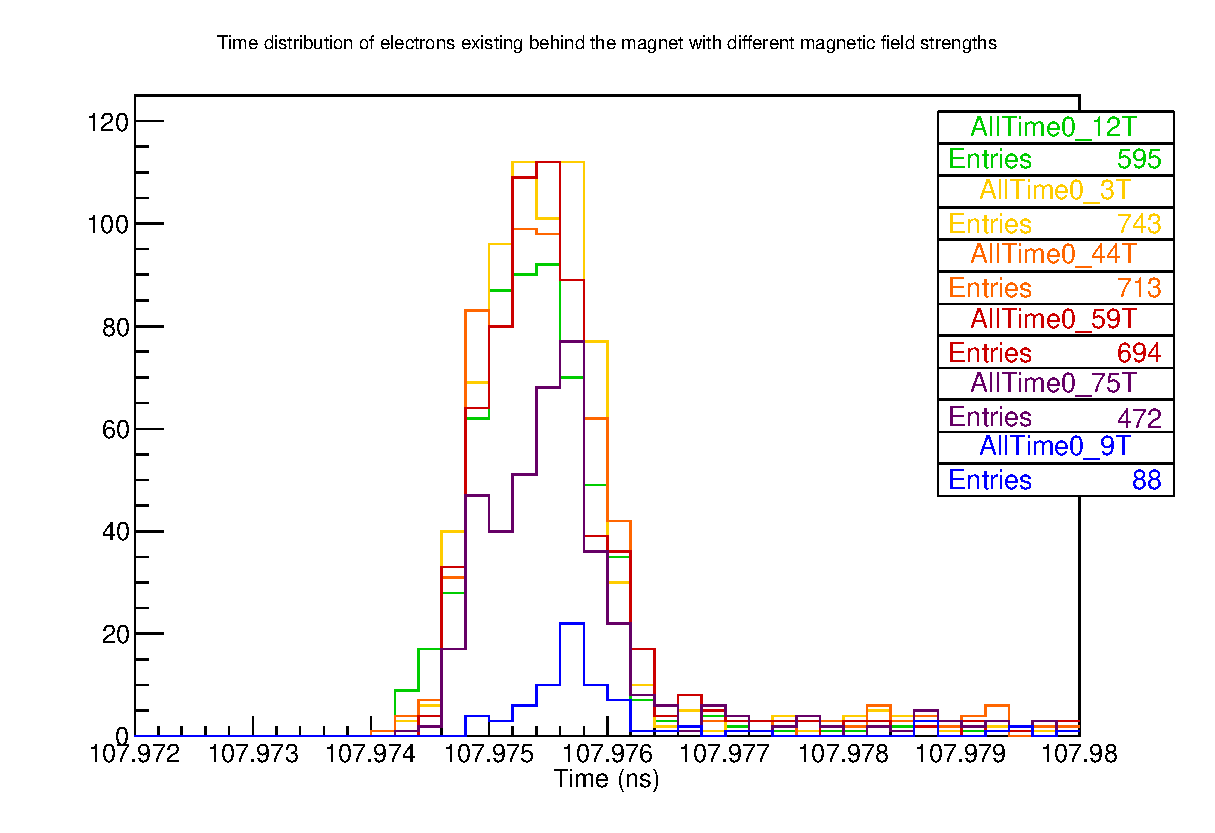
\includegraphics[width=0.8\textwidth]{T_Canvas_different_B.eps}
  \caption[The time distribution of the test beam generation for test beam line 21.]{The time distribution of the test beam generation for the test beam line 21 is the time between the start of the simulation with the DESY-II beam bunch hitting the primary target and the test beam particles entering the test beam area. The simulation of the test beam was done 200 times for six different magnetic field strengths between B\,=\,0.12\,T and 0.9\,T.}
    \label{fig:testbeam_time}
\end{figure}

Since the beam is collimated twice, the Gaussian energy distributions are narrow. Measured distributions have a width of about 5\,\%. 

\begin{table}[ht]
  \begin{center}
    \begin{tabular}{|c|c|c|r@{.}l|}
    \cline{1-5}
    \arraybackslash\textbf{B (T)} & \multicolumn{1}{>{\centering\arraybackslash}m{1.5cm}|}{\textbf{Mean energy (GeV)}} & \multicolumn{1}{>{\centering\arraybackslash}m{1.5cm}|}{$\sigma$ (GeV)} & \multicolumn{2}{>{\centering\arraybackslash}m{1.5cm}|}{\textbf{Energy spread (\%)}}\\ 
    \hline
    \hline
    0.12 & 0.907 & 0.116 & 12&752\\ 
    \hline
    0.30 & 2.162 & 0.197 & 9&112\\ 
    \hline
    0.44 & 3.001 & 0.111 & 3&705 \\
    \hline
    0.59 & 3.989 & 0.128 & 3&201\\
    \hline
    0.75 & 5.078 & 0.163 & 3&202\\
    \hline
    0.90 & 6.003 & 0.093 & 1&542\\
    \hline
    \end{tabular}
  \end{center}
  \caption{Table of the final results for the particle energy and its spread for the final test beam (cf. Figure~\ref{fig:E_different_B}). The results are gained from 200 full simulations for each magnetic field strength.}
  \label{table:energy_spreads}
\end{table}

Additionally, the linear dependency between the magnetic field strength of the 
test beam magnet and the particle energy is shown for a comparison to the plot 
in Figure~\ref{fig:p_over_I}.

\begin{figure}[htbp!]
  \centering
  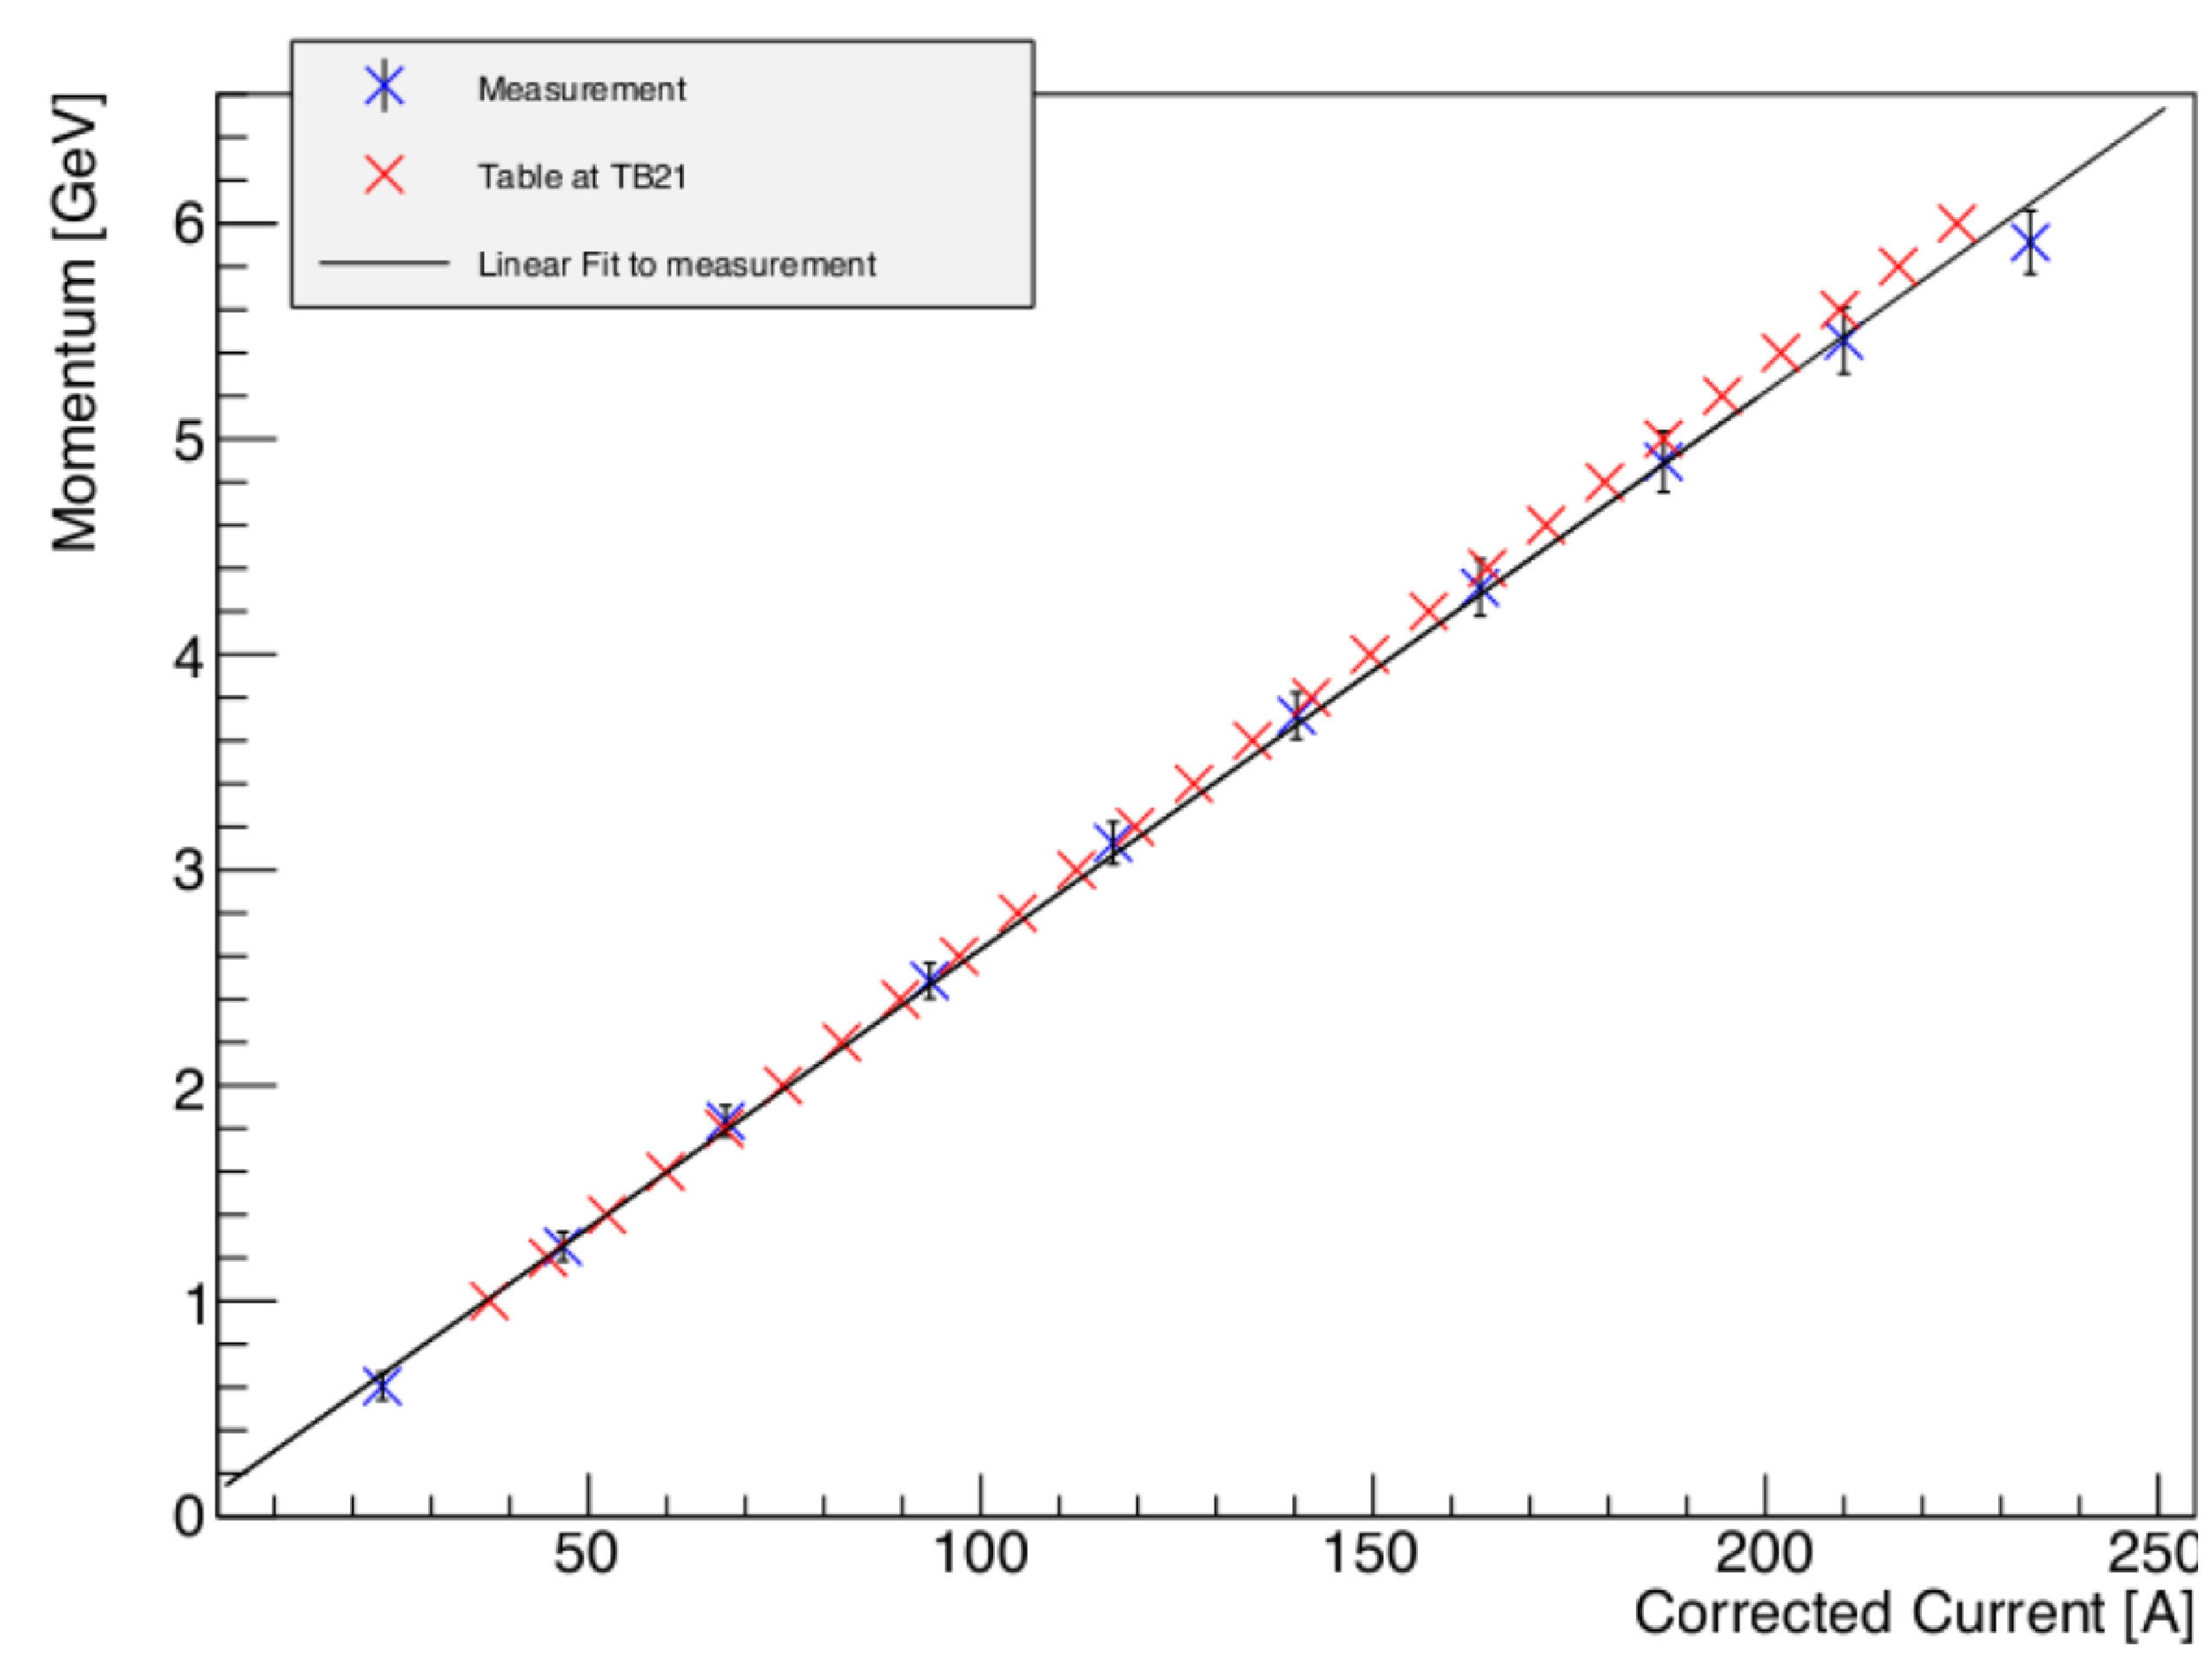
\includegraphics[width=0.5\textwidth]{Momentum_over_I.eps}
  \caption[Plot of the particle momentum in dependency of the current through the test beam magnet.]{Plot of the particle momentum as a function of the current through the MR dipole magnet of the test beam line 21.~\cite{Paul}}
    \label{fig:p_over_I}
\end{figure}

Figure~\ref{fig:E_different_B} shows the energy distributions for six different 
magnetic field strengths between 0.12\,T and 0.9\,T. With the given statistics, 
the distributions have a spread of 1.5\% - 12.8\%.\\An interesting point is that 
for all magnetic field strengths, there is a small number of particles with 
energies below 0.5\,GeV. In Figure~\ref{fig:TBCollimator_rate} (b) which shows 
the added up distributions of the particle energy, this leads to a significant 
count of particles with energies of 1\,GeV and lower. When a cut is applied on 
the simulated data such that only particles with energies of the mean value$\pm 
\sigma$ from the single energy distribution fits are taken into account, the 
plot of the particle count in dependency on their energy becomes a Gaussian 
distribution (see Figure~\ref{fig:TBCollimator_rate} (a)) as expected from 
Figure~\ref{fig:TB_secondary_target_rates}. However, 
Figure~\ref{fig:TB_secondary_target_rates} only shows the expected rate for a 
certain particle energy. The simulation indicates that there are always 
particles with energies smaller than 0.5\,GeV, because of particle interactions 
with the collimator and shielding material. The rate for particles with energies 
smaller than 1\,GeV is therefore higher than expected, as shown is 
Figure~\ref{fig:TBCollimator_rate} (a). 

\begin{figure}[ht]
  \centering
  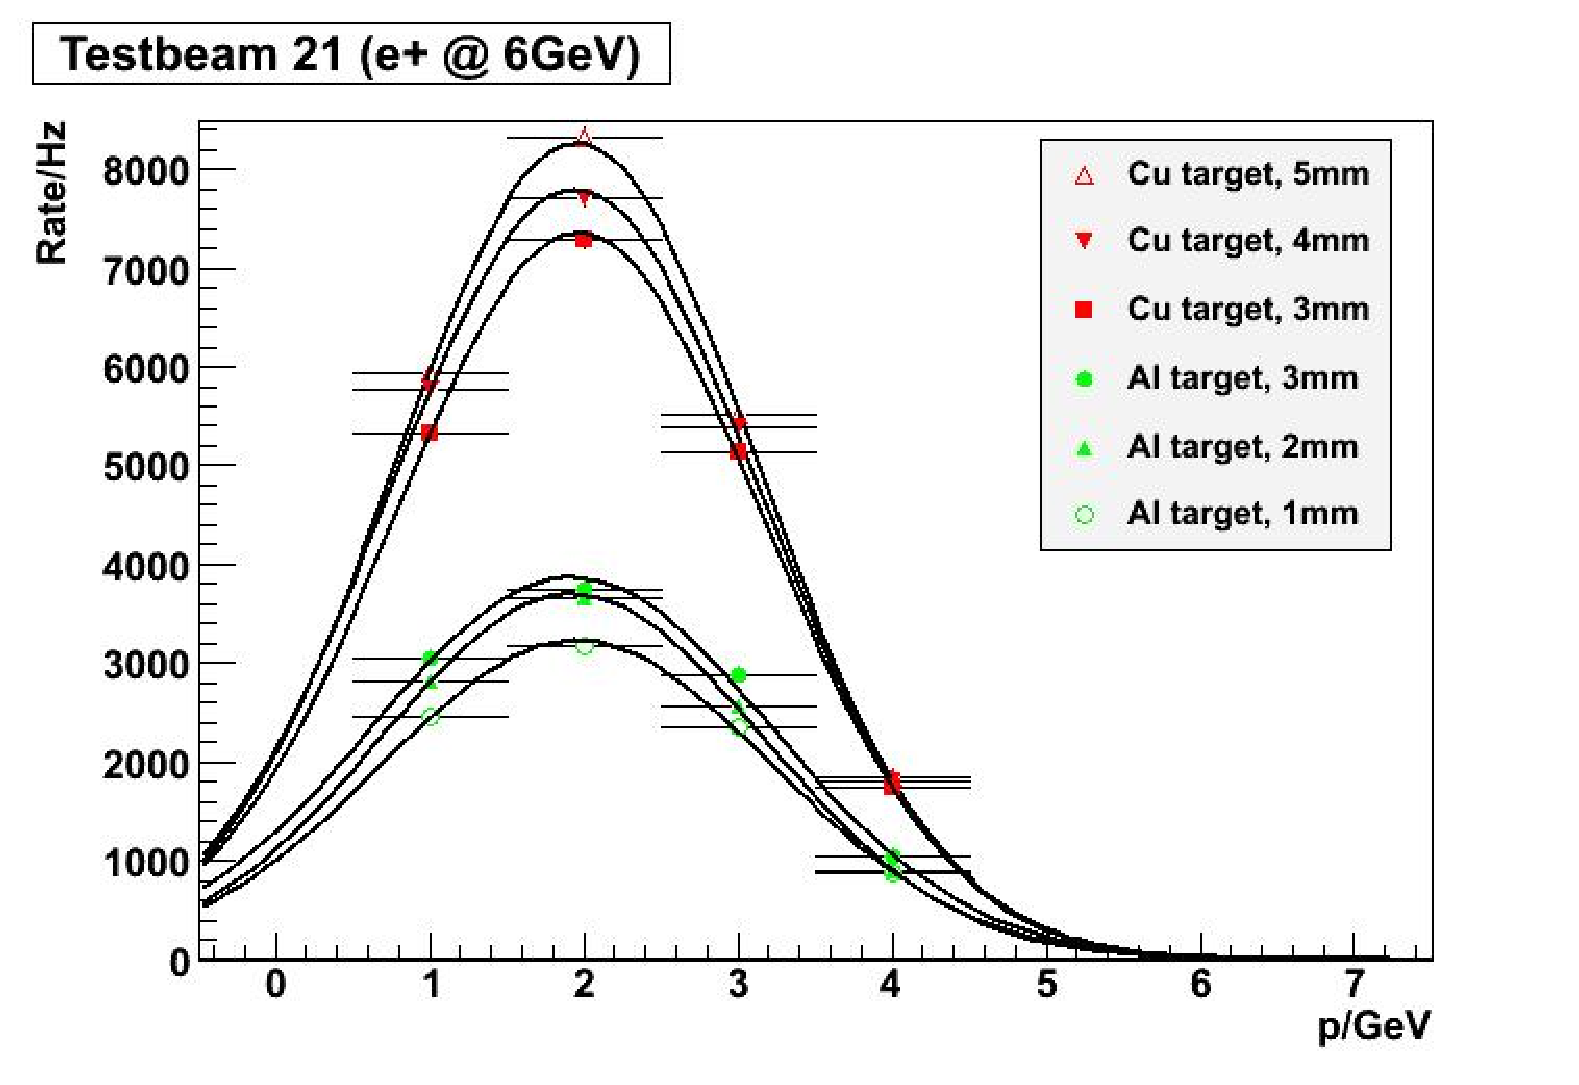
\includegraphics[width=0.55\textwidth]{TB_secondary_target_rates.eps}
  \caption[Test beam rate dependency on properties of secondary target.]{The measured rate of the positron beam for test beam line 21 is plotted as a function of the particle momentum. The rate is highly dependent on the material and thickness of the secondary target. In general, the thicker the material, the higher the conversion rate. Additionally, copper yields higher rates than aluminium, since the cross section for pair production is greater for copper than for aluminium.}
    \label{fig:TB_secondary_target_rates}
\end{figure}

\begin{figure}[H]
  \centering
  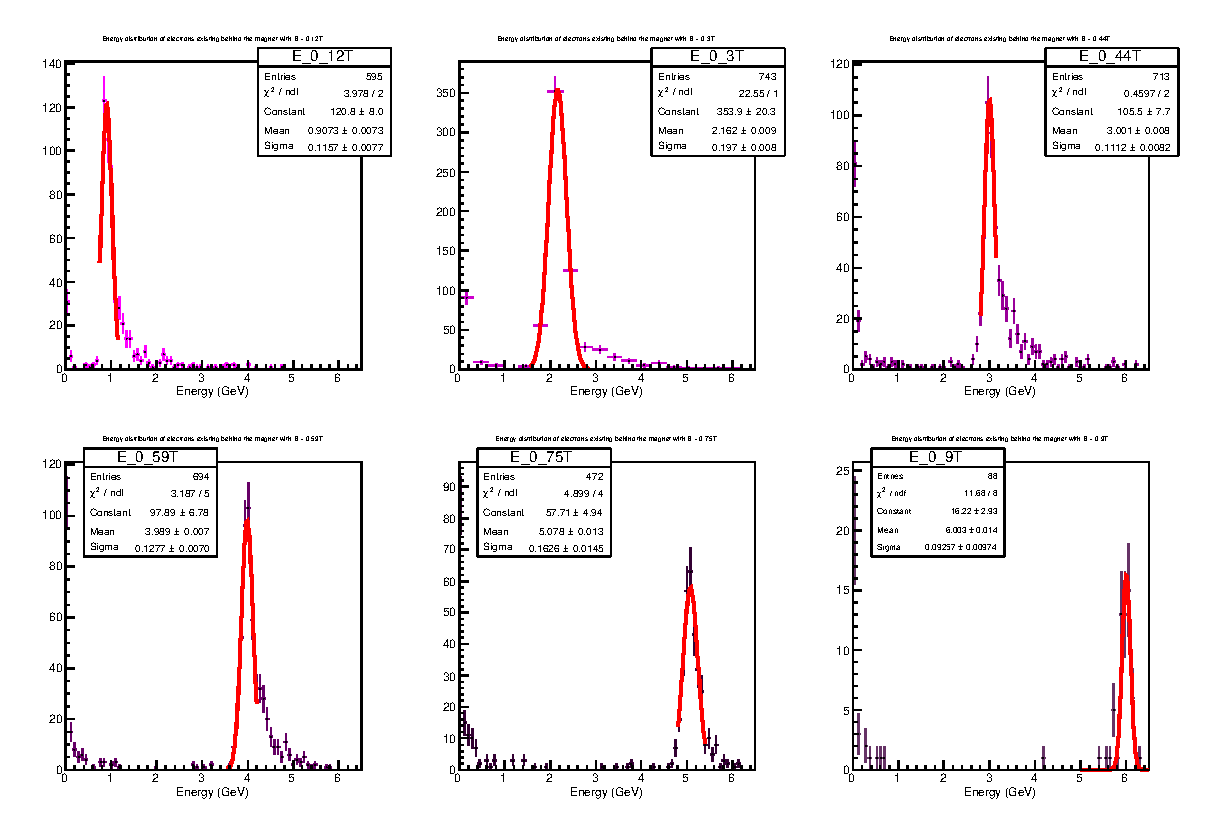
\includegraphics[width=\textwidth]{E_Canvas_different_B.eps}
  \caption[Plot of the simulated energy distributions for different magnetic field strengths.]{Plots of the energy distributions of the simulated test beam for different magnetic field strengths of the dipole magnet of the test beam line 21. The magnetic field strengths range from 0.12\,T to 0.9\,T. For each plot, the full simulation of the test beam line was repeated 200 times, so that the distributions are directly comparable.}
    \label{fig:E_different_B}
\end{figure}

\begin{figure}
  \centering
  \begin{subfigure}[t]{0.49\textwidth}
    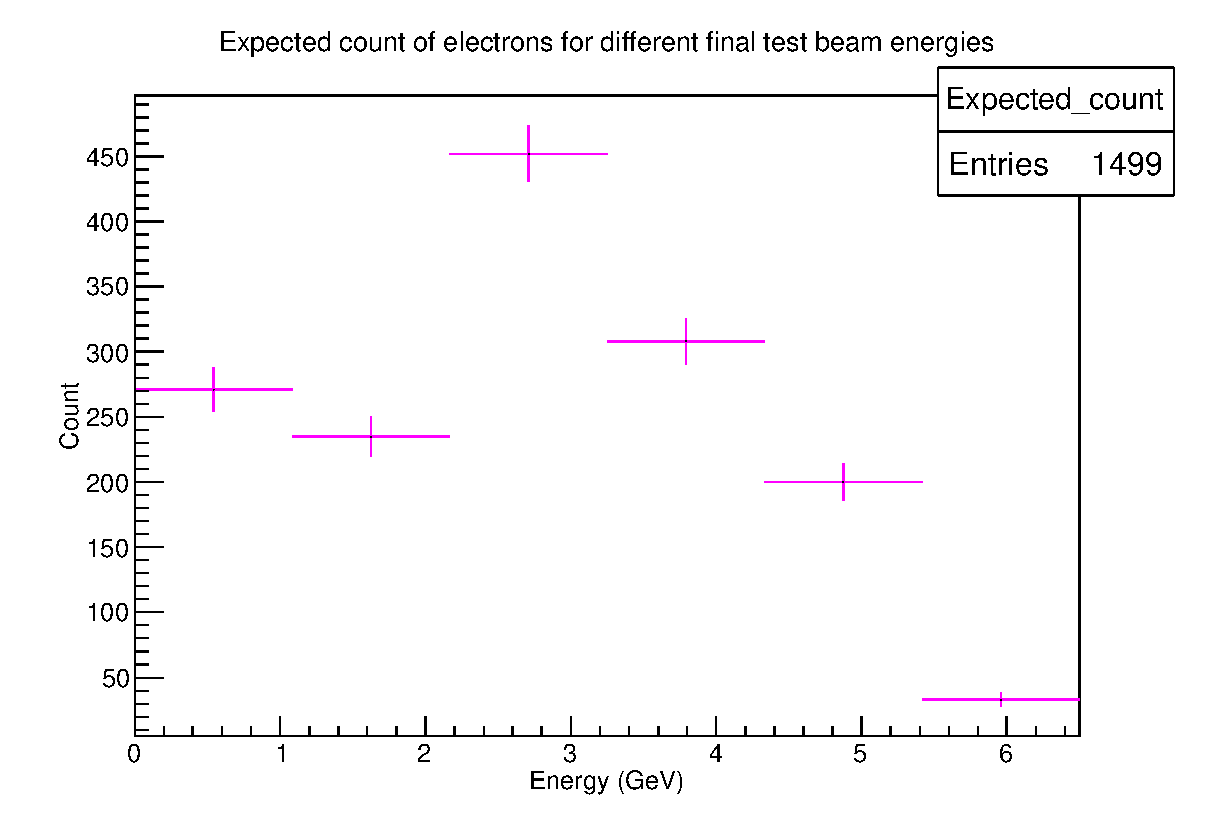
\includegraphics[width=\textwidth]{Rate_Energy.eps}
      \caption{}
  \end{subfigure}
\hfill
  \begin{subfigure}[t]{0.49\textwidth}
    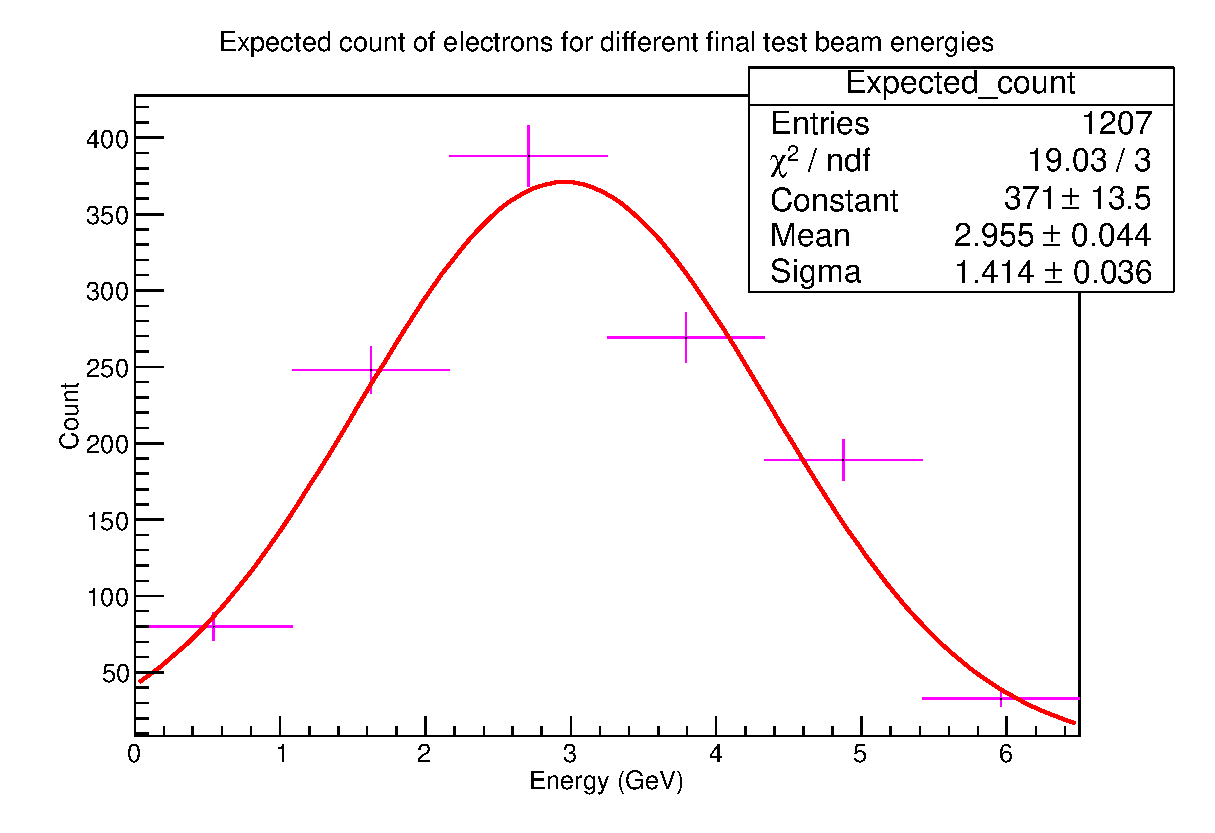
\includegraphics[width=\textwidth]{Rate_Energy_Cut.eps}
      \caption{}
  \end{subfigure}
 \caption[Plots of the test beam rate after the final collimation.]{Plots of the electron count in the test beam area after the final collimation with respect to the electron energy. Figure (a) shows a plot of the added up energy distributions of Figure~\ref{fig:E_different_B} for the six different magnetic field strengths. Due to the count of particles with energies smaller than 0.5\,GeV, Figure (a) shows a higher count of particles with energies up to 1\,GeV than expected. When a cut is applied on the particle energy for the first bin such that only particles with energies around the mean value of the energy distribution (from Figure~\ref{fig:E_different_B}) contribute to the distribution, the particle count is Gaussian distributed (Figure (b)).}
  \label{fig:TBCollimator_rate}
\end{figure}

As the DESY-II beam bunch hits the primary targets of the test beam lines with a 
rate of 1\,MHz, the particle counts shown here in 
Figures~\ref{fig:E_different_B} and \ref{fig:TBCollimator_rate} have to be 
scaled up with a factor of 5\,000\,Hz ($\frac{1\,\mathrm{MHz}}{200}$). This 
leads with a maximum count of about 350 simulated particles (for 200 simulated 
DESY-II beam bunches) to a maximum rate of about 1,750,000\,Hz. The discrepancy 
to the measured rates in the test beam area could be due to the fact that the 
simulated rate is given directly behind the final collimator, whereas the 
measured rates were measured in the test beam area metres away from the 
collimator. Because the final test beam widens isotropically, only a fraction of 
the beam was measured. Further investigations on the beam rates are necessary to 
explain this large discrepancy.

Finally, the particle energy is plotted over the magnetic field strength (see 
Figure~\ref{fig:E_over_B}). The plot is a profile plot and shows the average 
energy of the final test beam for a certain magnetic field strength of the 
dipole magnet. Hence, one can read from the figure which beam energy is to be 
expected, when a specific magnetic field strength is set for the test beam 
magnet. The relationship between the energy and the field strength is linear.

\begin{figure}[!ht]
  \centering
  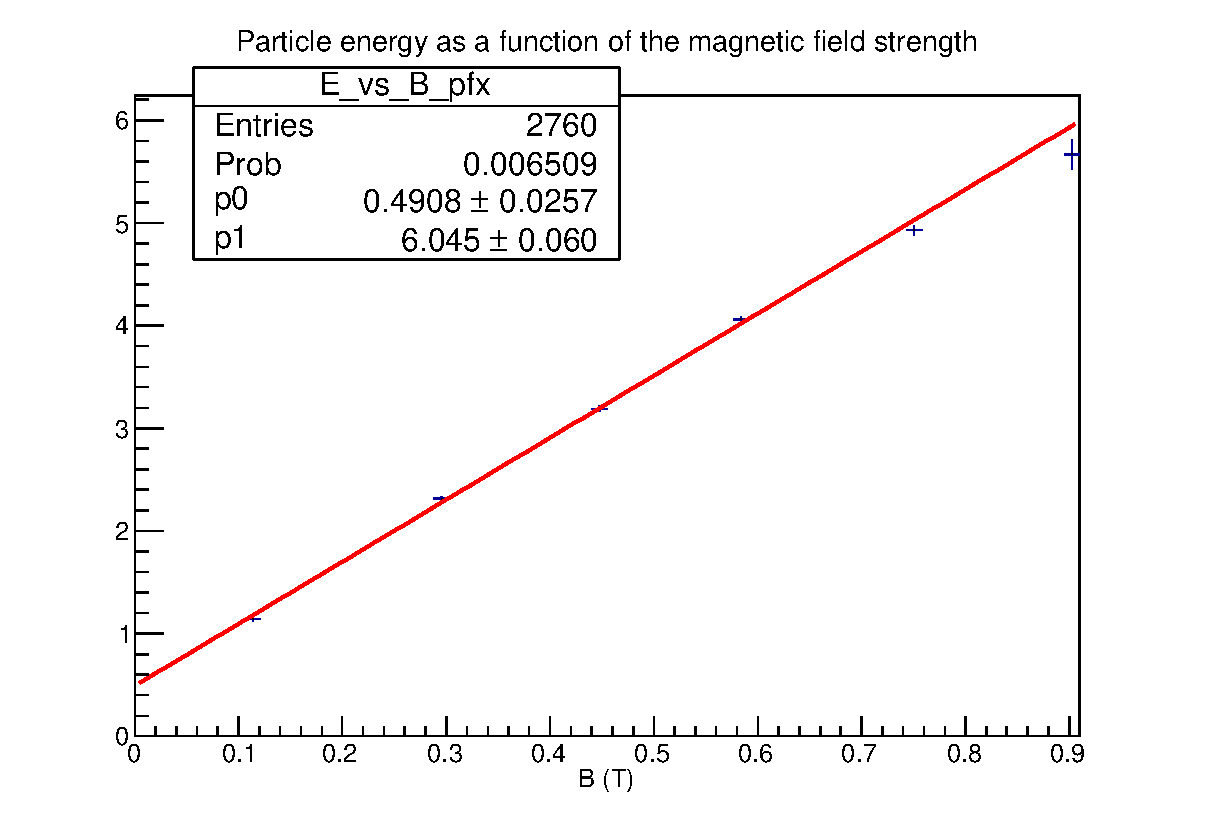
\includegraphics[width=0.9\textwidth]{E_vs_B_Canvas.eps}
  \caption[Plot of the simulated particle energy in dependency of the magnetic field strength.]{Profile plot of the particle energy of the simulated test beam as a function of the magnetic field strength of the dipole magnet of the test beam line 21. The plot shows the average energy for one magnetic field strength. As so far only six different magnetic field strengths were simulated, six average energies are plotted.}
    \label{fig:E_over_B}
\end{figure}

\begin{figure}[!ht]
  \centering
  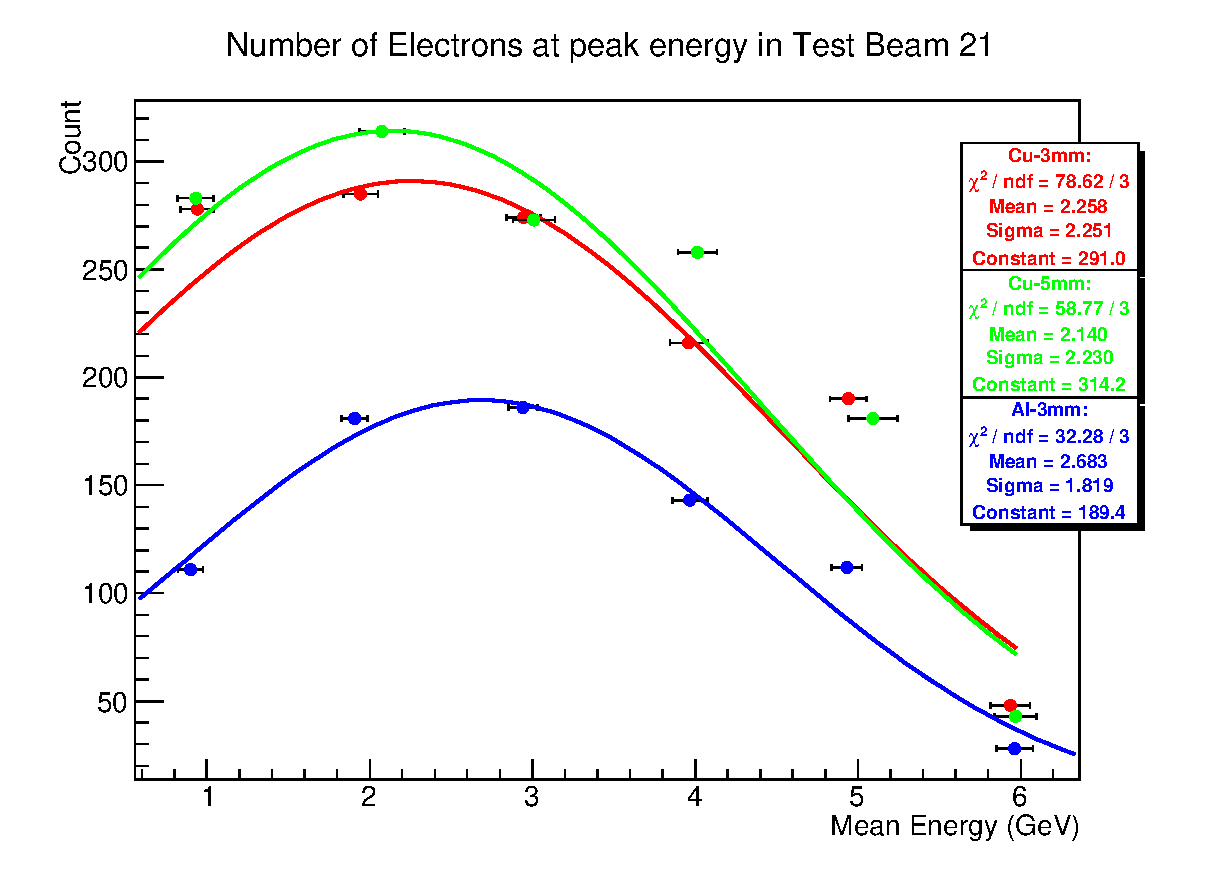
\includegraphics[width=\textwidth]{ElectronsPerPeakEnergyCombined.eps}
  \caption[Plot of the simulated particle count in dependency of the particle energy.]{The particle counts for the peak energy at six different magnetic field strengths are plotted as a function of the particle energy. As expected from Figure~\ref{fig:TB_secondary_target_rates} copper as the material for the secondary target of the test beam line yield higher rates than aluminium. The final test beam count peaks for energies between 2 and 3\,GeV.}
    \label{fig:N_over_E}
\end{figure}